\documentclass[conference]{IEEEtran}
\IEEEoverridecommandlockouts

% --- Packages -------------------------------------------------------------
\usepackage{cite}
\usepackage{amsmath}
\usepackage{newtxtext}
\usepackage{newtxmath}
\usepackage{array}
\usepackage{booktabs}
\usepackage{url}
\usepackage{xcolor}
\usepackage{tikz}
\usetikzlibrary{arrows.meta,positioning,calc}
\usepackage[hidelinks]{hyperref}

\hyphenpenalty=10000
\exhyphenpenalty=10000
\tolerance=9999
\emergencystretch=3em

\usepackage{etoolbox}
\patchcmd{\abstract}{\textit{\abstractname}---\relax}{\textit{\abstractname}:\ }{}{}
\patchcmd{\IEEEkeywords}{\textit{\IEEEkeywordsname}---\relax}{\textit{\IEEEkeywordsname}:\ }{}{}

\newcommand{\code}[1]{\texttt{\small #1}}

\tikzset{
  lbox/.style={draw, rounded corners=2pt, align=center, font=\scriptsize,
               text width=18mm, minimum height=9mm, inner sep=2pt, fill=blue!5},
  iobox/.style={lbox, fill=black!8},
  cbox/.style={lbox, fill=green!8},
  obox/.style={draw, rounded corners=2pt, align=center, font=\scriptsize,
               text width=20mm, minimum height=10mm, inner sep=2pt, fill=green!8},
  centerbox/.style={draw, rounded corners=2pt, align=center, font=\scriptsize,
               text width=21mm, minimum height=13mm, inner sep=3pt, fill=blue!8},
  flow/.style={-{Latex[length=2mm]}, semithick},
}

\title{Capability Receipts for Auditable AI Agent Execution: A Design Science Study of Lattice}

\author{\IEEEauthorblockN{Lakshman Turlapati}
\IEEEauthorblockA{Independent Researcher\\
Email: lakshmanturlapati@gmail.com}}

\begin{document}

\maketitle

\begin{abstract}
Organizations increasingly deploy large language model systems that route work
across model providers, tools, files, modalities, and agent loops. These systems
produce operational traces, yet the traces are usually not sufficient for audit:
they can be edited after the fact, they often omit why a model was selected, they
do not bind inputs to outputs, and they rarely support offline replay by a party
that was not present during execution. This paper presents Lattice, a design
science artifact for auditable AI agent execution. Lattice introduces
\emph{capability receipts}: canonical, redacted, signed, and replayable records
of AI runs that capture intent, policy, routing, artifacts, invariants, outputs,
cost, latency, and verification metadata. The paper makes two contributions.
First, it defines a capability-receipt framework for signed, replayable, and
policy-enforced execution across model and agent workflows. Second, it develops
an organizational auditability model showing how capability receipts strengthen
governance, accountability, reproducibility, and control compared with ordinary
logs, observability traces, and provider wrappers. The artifact combines
deterministic routing, terminal policy tripwires, tamper-evident signing,
content-addressed replay, cross-language conformance vectors, and chained
multi-agent provenance. Evaluation is presented through design requirements,
implementation evidence, conformance checks, replay scenarios, tripwire tests,
and an audit workflow. The result is a practical control layer that turns
auditability from an external after-the-fact activity into a built-in property
of each AI run.
\end{abstract}

\begin{IEEEkeywords}
AI governance, AI auditability, design science research, capability receipts,
agent execution, digital accountability, replayable systems, software provenance
\end{IEEEkeywords}

\section{Introduction}

AI applications are moving from narrow text-generation tasks into operational
systems that triage work, extract information from documents, call tools, route
between model providers, and coordinate agent loops. In these systems, a single
business task may include prompts, files, images, JSON, model-selected tool
calls, provider fallbacks, policy constraints, and multiple child agents. This
creates a governance problem. The organization needs to know not only what the
system returned, but also what it was asked to do, which model path was chosen,
which constraints were applied, whether a policy violation stopped execution,
and whether the record can be verified later.

Most production stacks answer these questions with logs, traces, dashboards, or
model-provider metadata. Those mechanisms are useful for operations, but they
are weak audit evidence. A log line can be edited. A trace may document latency
without proving the integrity of the input-output relationship. A provider
wrapper may normalize APIs without recording a deterministic reason for model
selection. An agent framework may show a tool sequence without producing a
portable artifact that an external reviewer can verify with a public key. The
result is a gap between responsible-AI principles and the operational evidence
needed to demonstrate that a particular run complied with organizational policy.

The information systems literature has long treated IT artifacts as objects that
can encode organizational intent and control \cite{hevner2004dsr,gregor2013dsr}.
The AI governance literature similarly emphasizes accountability,
transparency, human oversight, and operationalization of principles
\cite{jobin2019global,berente2021managingai,raji2020accountability}. Yet a
concrete design question remains underdeveloped: what should an AI-agent
runtime emit so that a later reviewer can verify a run without trusting the
operator's unstructured logs?

This paper addresses that question through Lattice, a TypeScript-first runtime
and protocol artifact for auditable AI execution. Lattice is capability-first:
a developer describes the job, provides artifacts, declares desired outputs, and
sets policy constraints. The runtime routes the work using an inspectable
deterministic policy, executes the run, evaluates output invariants, and emits a
signed capability receipt. The receipt is canonicalized, redacted before
signing, signed inside a Dead Simple Signing Envelope (DSSE), and paired with
content-addressed artifacts for offline replay.

The research question is:

\begin{quote}
How can an AI-agent runtime produce portable, verifiable audit evidence for
individual model and agent runs while preserving deterministic policy
enforcement and replayability?
\end{quote}

The paper makes two explicit contributions.

\begin{enumerate}
\item \textbf{Capability-receipt framework.} The paper defines capability
receipts as a design primitive for signed, replayable, policy-enforced AI
execution. A receipt binds run intent, route selection, policy constraints,
redaction, output hashes, and verification metadata into a tamper-evident
artifact.
\item \textbf{Organizational auditability model.} The paper maps receipt
mechanisms to organizational control needs: governance evidence, accountability
for routing and tool use, reproducibility through offline replay, and control
through terminal tripwires that fail closed instead of retrying unsafe outputs.
\end{enumerate}

The novelty is not that digital signatures, canonical JSON, software
provenance, model cards, or runtime traces are individually new. The novelty is
their integration into a runtime-level audit artifact for AI-agent execution:
deterministic routing explains why a model was selected; policy tripwires make
unsafe outputs terminal; DSSE signing makes the run record tamper-evident;
content-addressed replay allows independent verification; and chained receipts
represent multi-agent provenance.

\begin{figure*}[t]
\centering
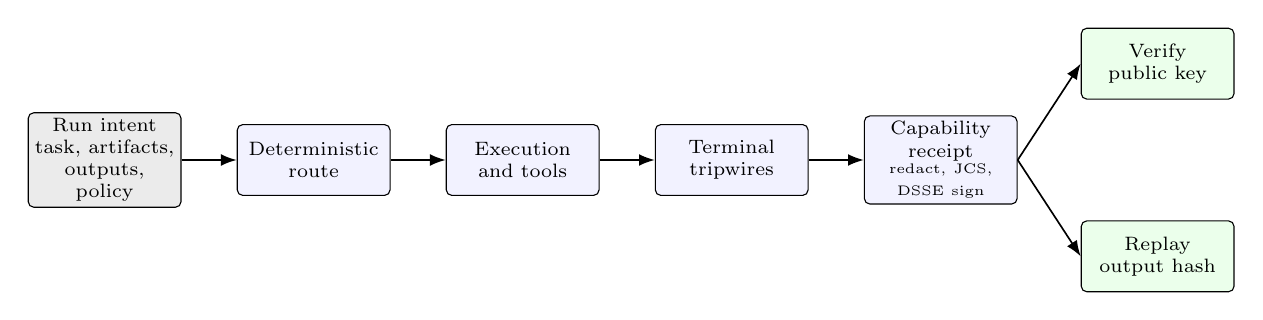
\begin{tikzpicture}[node distance=6mm and 7mm]
  \node[iobox] (intent) {Run intent\\ task, artifacts,\\ outputs, policy};
  \node[lbox, right=of intent] (route) {Deterministic\\ route};
  \node[lbox, right=of route] (exec) {Execution\\ and tools};
  \node[lbox, right=of exec] (trip) {Terminal\\ tripwires};
  \node[lbox, right=of trip] (receipt) {Capability\\ receipt\\ \tiny redact, JCS,\\ \tiny DSSE sign};
  \node[cbox, above right=2mm and 8mm of receipt] (verify) {Verify\\ public key};
  \node[cbox, below right=2mm and 8mm of receipt] (replay) {Replay\\ output hash};
  \draw[flow] (intent) -- (route);
  \draw[flow] (route) -- (exec);
  \draw[flow] (exec) -- (trip);
  \draw[flow] (trip) -- (receipt);
  \draw[flow] (receipt.east) -- (verify.west);
  \draw[flow] (receipt.east) -- (replay.west);
\end{tikzpicture}
\caption{Lattice audit evidence lifecycle. A capability-first run is routed by a
deterministic decision function, executed under policy, stopped by terminal
tripwires when needed, and committed to a signed receipt that can be verified
and replayed offline.}
\label{fig:lifecycle}
\end{figure*}

\section{Literature Review}

\subsection{Design Science Research in Information Systems}

Design science research (DSR) studies purposeful artifacts that solve relevant
organizational problems while contributing generalizable design knowledge
\cite{march1995design,hevner2004dsr,peffers2007dsrm}. The DSR tradition is
appropriate here because the core problem is not only descriptive. Organizations
need a buildable artifact that changes the evidence available after AI
execution. Following Gregor and Hevner \cite{gregor2013dsr}, the paper positions Lattice as both
an instantiation and a source of design principles for auditability: make run
intent explicit, make route choice deterministic, make unsafe outputs terminal,
bind records cryptographically, and support replay by a party outside the live
execution environment.

\subsection{Responsible AI Governance and Accountability}

Responsible AI guidelines converge on principles such as transparency,
accountability, privacy, robustness, fairness, and human oversight
\cite{jobin2019global,floridi2018ai4people,nistairmf}. The challenge is
operationalization. Recent information systems work argues that AI governance
requires structural, relational, and procedural practices rather than abstract
principles alone \cite{berente2021managingai}. Algorithmic accountability work
also shows that audit claims require traceability and evidence about the
decisions made during system operation \cite{diakopoulos2016accountability,
wieringa2020accounting,kroll2021traceability}. Lattice contributes at this
operational layer. It does not replace governance policy; it provides a
verifiable record that a governance process can inspect.

\subsection{Algorithmic and Internal Auditing}

Auditing research emphasizes evidence, control, independence, and the risk that
organizational systems produce reports that cannot be independently verified
\cite{power1997audit}. In AI systems, the accountability gap is amplified by
opaque models, evolving prompts, nondeterministic outputs, and external
providers. Raji et al. \cite{raji2020accountability} propose internal algorithmic auditing
as an end-to-end accountability process. Lattice addresses a complementary
technical question: what runtime evidence should such a process consume? A
capability receipt is designed to be a stable audit object rather than a
dashboard view or mutable operational trace.

\subsection{Software Provenance and Reproducibility}

The software supply-chain community has developed mature mechanisms for signed
provenance. in-toto signs the steps that produce software artifacts
\cite{intoto}; DSSE defines an envelope for unambiguous payload signing
\cite{dsse}; SLSA defines supply-chain integrity levels \cite{slsa}; and
Sigstore makes software signing more accessible \cite{sigstore}. Lattice
adapts this lineage from build artifacts to runtime AI work. The signed object
is not a compiled binary; it is a single AI run. Reproducibility literature in
machine learning similarly emphasizes that claims should be checkable and
repeatable \cite{reproml,sculley2015debt}. Lattice narrows this to run-level
replay: it does not claim to reproduce a provider's future nondeterministic
behavior, but it verifies that the recorded run, artifacts, and output hash
match the signed receipt.

\subsection{Documentation, Transparency, and Observability}

Model Cards and Datasheets for Datasets improve disclosure about models and
datasets \cite{modelcards,datasheets}. Observability systems and agent
frameworks expose traces, spans, sessions, and tool calls. Provider wrappers and
agent frameworks such as the Vercel AI SDK, LangChain/LangGraph, LiteLLM, the
OpenAI Agents SDK, and the Model Context Protocol normalize development
interfaces \cite{vercelaisdk,langchain,litellm,openaiagents,mcp}. These
systems are complementary, but their core artifact is not a signed, portable,
replayable run receipt. The gap is therefore not visibility in the broad sense.
It is verifiable audit evidence for a specific AI execution.

\section{Design Science Method}

The study follows a DSR process with five activities adapted from established
DSR guidance \cite{hevner2004dsr,peffers2007dsrm,gregor2013dsr}. First, the
problem is identified as insufficient audit evidence for AI-agent execution.
Second, objectives are derived from governance and provenance needs. Third, the
artifact is designed and implemented as Lattice. Fourth, the artifact is
evaluated through executable invariants, conformance vectors, replay scenarios,
and audit workflows. Fifth, the artifact and design knowledge are communicated
through the manuscript and accompanying protocol documentation.

The artifact is evaluated as an operational control layer, not as a model
accuracy benchmark. This distinction matters. The relevant question is whether
the runtime produces evidence that can be verified, replayed, and used in
governance review. Latency and model quality depend on external providers and
are outside the receipt trust boundary.

\begin{table}[t]
\centering
\caption{Design requirements for auditable AI-agent execution.}
\label{tab:requirements}
\small
\begin{tabular}{@{}>{\raggedright\arraybackslash}p{0.17\linewidth}>{\raggedright\arraybackslash}p{0.46\linewidth}>{\raggedright\arraybackslash}p{0.27\linewidth}@{}}
\toprule
Requirement & Rationale & Lattice mechanism \\
\midrule
DR1 Intent & Auditors need to know what the system was asked to do. & Capability-first run model \\
DR2 Routing & Model choice should be explainable and reproducible. & Pure routing function and execution plan \\
DR3 Enforcement & Unsafe outputs should fail closed. & Terminal tripwires and contracts \\
DR4 Integrity & Run records must be tamper-evident. & Redact, canonicalize, DSSE sign \\
DR5 Replay & Reviewers need offline verification. & Content-addressed replay envelope \\
DR6 Lineage & Multi-agent work needs parent-child accountability. & Chained receipts and lineage fields \\
\bottomrule
\end{tabular}
\end{table}

Table~\ref{tab:requirements} summarizes the design requirements and the
mechanisms that implement them. These requirements are intended to be reusable
design knowledge for systems that need auditability even if they do not adopt
the Lattice implementation.

\section{Artifact Design}

\subsection{Capability-First Run Model}

Lattice begins with an intent rather than a provider call. A run declares a task,
artifacts, desired outputs, schemas, policies, and optional contracts. Artifacts
can include text, JSON, images, documents, audio, or tool results. Policies
express provider constraints, privacy classes, latency preferences, and budget.
This design shifts the unit of control from ``call this model'' to ``perform
this capability under these constraints.'' The receipt can therefore record the
organization's declared intent next to the runtime's actual route and outcome.

\subsection{Deterministic and Inspectable Routing}

Routing is implemented as a pure function over the capability catalog, request,
and policy. It performs hard filters, policy filters, stable scoring, and
deterministic tie breaking. The route decision records accepted candidates,
rejected candidates, fallback options, and typed reasons when no route is
possible. This makes model choice reviewable. An auditor can inspect why a
provider was selected and whether alternatives were rejected for capability,
privacy, budget, or policy reasons.

\subsection{Policy Tripwires with Terminal Semantics}

Output invariants act as tripwires. Examples include requirements to cite an
artifact, avoid personally identifiable information, or match a declared schema.
The important design choice is terminal semantics: when a tripwire fires, the
fallback chain is forbidden from retrying the run. This prevents a common unsafe
pattern in which a system keeps trying until a policy-violating output happens
to pass. For auditability, the receipt records the terminal outcome rather than
hiding it behind a later successful retry.

\subsection{Capability Receipts}

The capability receipt is the central artifact. A receipt is assembled from the
run record, redacted, canonicalized using the JSON Canonicalization Scheme
\cite{rfc8785}, and signed using Ed25519 \cite{rfc8032} inside a DSSE envelope
\cite{dsse}. The ordering is deliberate: redaction occurs before signing so
that secrets and detected personal information do not enter the signed bytes.
The receipt includes the run identifier, route, model class where available,
policy metadata, output hash, usage, cost, latency, redaction manifest, and key
identifier. Verification rejects unsupported or downgraded schema versions
before cryptographic work, reducing the risk that an older receipt shape can
bypass newer integrity commitments.

\subsection{Offline Replay and Content Addressing}

Receipts become stronger audit evidence when they can be replayed. Lattice pairs
receipts with content-addressed artifacts and materializes a replay envelope
only after verifying the receipt. This verify-before-load ordering prevents a
tampered receipt from triggering artifact loads or downstream side effects.
Replay reconstructs the recorded run and recomputes the output hash. It does not
claim to reproduce a provider's future model behavior; it verifies the integrity
of the recorded execution.

\subsection{Chained Multi-Agent Provenance}

Agent workflows add another audit problem: a parent agent may delegate work to
child agents, each of which calls tools or models. Lattice represents this with
chained receipts. Child receipts can include a parent receipt content identifier
and lineage metadata, allowing a reviewer to reconstruct a tree of delegated
work. This is the agent-execution analogue of provenance chains in software
supply-chain systems.

\section{Organizational Auditability Model}

The organizational value of capability receipts can be summarized as four forms
of auditability.

\begin{enumerate}
\item \textbf{Governance auditability.} A receipt records the policy and
contract context that governed a run. This helps a governance team evaluate
whether a run was performed under approved constraints.
\item \textbf{Accountability auditability.} A receipt records route selection,
tool use, parent-child receipt links, and typed failure reasons. This creates an
accountability chain for model and agent decisions.
\item \textbf{Reproducibility auditability.} A receipt and its content-addressed
artifacts support offline replay and output-hash comparison.
\item \textbf{Control auditability.} Terminal tripwires and verification errors
make policy enforcement visible as an auditable event rather than an internal
implementation detail.
\end{enumerate}

\begin{figure}[t]
\centering
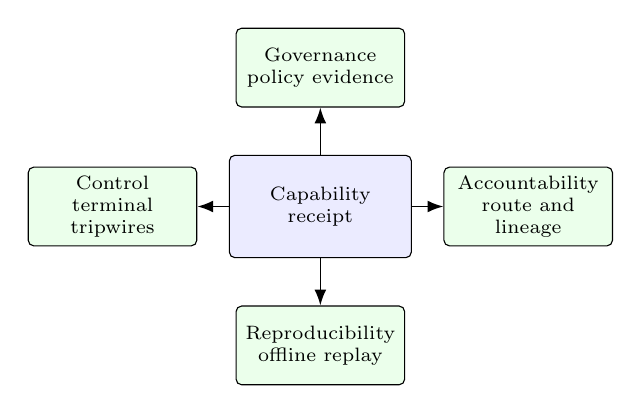
\begin{tikzpicture}[node distance=6mm and 4mm]
  \node[centerbox] (receipt) {Capability\\ receipt};
  \node[obox, above=of receipt] (gov) {Governance\\ policy evidence};
  \node[obox, right=of receipt] (acct) {Accountability\\ route and lineage};
  \node[obox, below=of receipt] (repro) {Reproducibility\\ offline replay};
  \node[obox, left=of receipt] (control) {Control\\ terminal tripwires};
  \draw[flow] (receipt) -- (gov);
  \draw[flow] (receipt) -- (acct);
  \draw[flow] (receipt) -- (repro);
  \draw[flow] (receipt) -- (control);
\end{tikzpicture}
\caption{Organizational auditability model. A receipt is the audit object that
connects technical execution evidence to governance, accountability,
reproducibility, and control review.}
\label{fig:auditability}
\end{figure}

Table~\ref{tab:comparison} contrasts this model with common alternatives.

\begin{table}[t]
\centering
\caption{Capability receipts compared with common evidence mechanisms.}
\label{tab:comparison}
\small
\begin{tabular}{@{}>{\raggedright\arraybackslash}p{0.25\linewidth}>{\raggedright\arraybackslash}p{0.30\linewidth}>{\raggedright\arraybackslash}p{0.33\linewidth}@{}}
\toprule
Mechanism & Strength & Audit limitation \\
\midrule
Application logs & Easy to collect and search & Mutable and rarely bind inputs to outputs \\
Observability traces & Strong operational visibility & Usually not portable signed evidence \\
Provider metadata & Useful billing and usage facts & Provider-specific and incomplete for policy \\
Agent transcripts & Explain step sequences & May omit route rationale and integrity checks \\
Capability receipts & Signed, replayable, policy-aware run record & Requires key management and artifact retention \\
\bottomrule
\end{tabular}
\end{table}

This model does not remove the need for organizational governance. It gives the
governance process a better object to inspect. A receipt can be attached to an
incident, reviewed during a control assessment, used as a regression fixture, or
sampled by an internal audit team.

\subsection{Illustrative Use Case: Aircraft Component Warranty Adjudication}

Aircraft-component warranty adjudication is a useful boundary case because the
evidence and decision authority are distributed across organizations. IATA
reports that warranty agreements and claim handling vary among original
equipment manufacturers (OEMs), maintenance suppliers, and airlines; its
guidance identifies part and serial numbers, time since new or overhaul, removal
reason and date, aircraft registration, and sometimes photographs as core claim
evidence \cite{iataWarranty2024}. More recently, IATA described maintenance data
as fragmented across airlines, maintenance, repair, and overhaul organizations
(MROs), OEMs, suppliers, and service providers, and linked warranty recovery to
connecting maintenance events, component performance, repair history, and
contractual terms \cite{iataWmes2026}. ICAO's electronic aircraft maintenance
records work foregrounds record integrity and transferability, while FAA
Advisory Circular 43-9D provides active guidance on maintenance record-making
and recordkeeping under 14 CFR parts 43 and 91 \cite{icaoEamr,faaAc439d}.

Consider, illustratively, an airline seeking recovery after the premature
removal of a serialized component. Its evidence set may contain part and serial
data, removal and installation records, aircraft telemetry, borescope images or
video, technician notes and voice material, prior repair history, maintenance
manual excerpts, and applicable warranty terms. These artifacts differ in
format, sensitivity, custody, and contractual relevance. Copying all of them
into a general-purpose model endpoint would create an unnecessary disclosure
surface and would still leave the resulting recommendation difficult to audit.

The airline or MRO first performs a \emph{restricted local run}. The capability
catalog exposes only an approved local or on-premises provider for restricted
data; a provider allow-list, \code{privacy: restricted}, \code{noUpload}, and
\code{noPublicUrl} constraints make that boundary explicit. Deterministic
routing rejects candidates that cannot satisfy it. The run does not decide the
claim. It produces typed findings---for example, an event chronology, extracted
part identifiers, measured values, and candidate failure observations---with
lineage back to the source artifacts. Its execution plan and receipt record the
selected route, rejected alternatives, transformations, input commitments, and
output commitment.

\begin{figure*}[t]
\centering
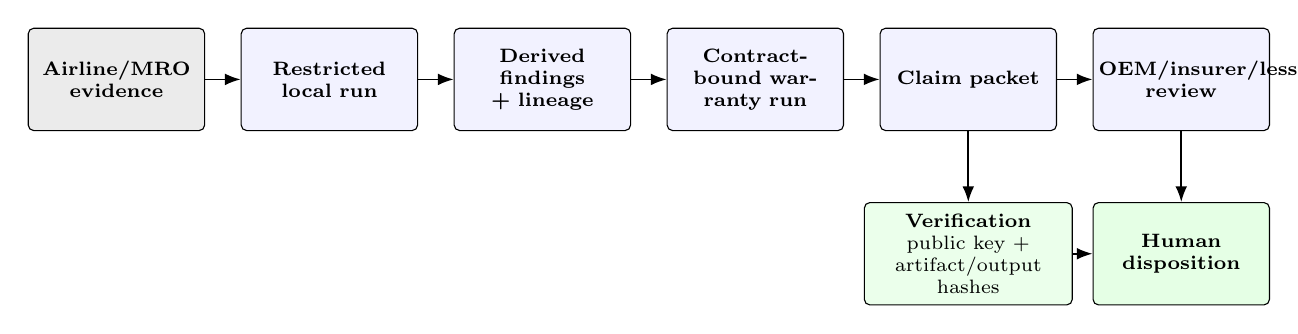
\begin{tikzpicture}[
  node distance=9mm and 4.5mm,
  warranty/.style={draw, rounded corners=2pt, align=center,
                   font=\scriptsize, text width=21mm, minimum height=13mm,
                   inner sep=2pt, fill=blue!5},
  verification/.style={draw, rounded corners=2pt, align=center,
                       font=\scriptsize, text width=25mm, minimum height=13mm,
                       inner sep=2pt, fill=green!8}
]
  \node[warranty, fill=black!8] (evidence) {\textbf{Airline/MRO evidence}};
  \node[warranty, right=of evidence] (local) {\textbf{Restricted local run}};
  \node[warranty, right=of local] (findings) {\textbf{Derived findings + lineage}};
  \node[warranty, right=of findings] (contract) {\textbf{Contract-bound warranty run}};
  \node[warranty, right=of contract] (packet) {\textbf{Claim packet}};
  \node[warranty, right=of packet] (review) {\textbf{OEM/insurer/lessor review}};
  \node[verification, below=of packet] (verify)
    {\textbf{Verification}\\public key +\\artifact/output hashes};
  \node[warranty, below=of review, fill=green!10] (human)
    {\textbf{Human disposition}};

  \draw[flow] (evidence) -- (local);
  \draw[flow] (local) -- (findings);
  \draw[flow] (findings) -- (contract);
  \draw[flow] (contract) -- (packet);
  \draw[flow] (packet) -- (review);
  \draw[flow] (packet) -- (verify);
  \draw[flow] (verify) -- (human);
  \draw[flow] (review) -- (human);
\end{tikzpicture}
\caption{Illustrative workflow for cross-organizational aircraft-component
warranty adjudication. The verification branch checks portable execution
evidence before human disposition. This is a design application, not a deployed
evaluation.}
\label{fig:aviation-warranty}
\end{figure*}

Only the derived findings and necessary evidence slices proceed to a second,
\emph{contract-bound warranty run}, as shown in
Figure~\ref{fig:aviation-warranty}. The contract binds the applicable warranty
terms, an output schema, approved providers, privacy constraints, and a cost
ceiling. Structured output can separate eligibility, supporting and contrary
evidence, contractual basis, uncertainty, and a recommended commercial action.
A \code{must-cite} tripwire requires evidence references, a
\code{field-from-table} tripwire restricts specified fields to values admitted
by the contractual table, and a \code{no-pii} tripwire prevents prohibited
personal-data patterns detected at the configured result path from entering the
shareable result. A violation is terminal:
Lattice records the failed control and does not try another model until one
happens to pass.

For a successful run, the operator assembles a portable claim packet containing
the recommendation, execution plan, signed receipt, necessary artifacts, and
replay evidence. An OEM, insurer, or lessor can use the public key and
artifact/output hashes to verify the signer and commitments, inspect why the
route was selected, and replay the recorded result without access to the
operator's live system. The mapping to the four auditability dimensions is
direct: policy and contract commitments support \emph{governance}; route
rationale and artifact lineage support \emph{accountability}; hashes and replay
support \emph{reproducibility}; and terminal tripwire verdicts support
\emph{control}. The packet informs review, but authorized engineering,
maintenance, commercial, and legal personnel retain authority over the final
warranty and maintenance disposition.

The assurance boundary is procedural. Lattice can prove that a signer bound a
specified execution procedure and output commitment to particular artifact
hashes, policy, route, and control verdict. It does not prove sensor accuracy,
the truth of maintenance records, media authenticity, model correctness,
regulatory compliance, or aircraft airworthiness. C2PA Content Credentials can
complement Lattice by carrying capture and edit provenance for images or video,
but C2PA likewise presents provenance assertions for human trust decisions
rather than deciding their truth \cite{c2pa2026}. Neither mechanism substitutes
for approved maintenance data, regulatory processes, or accountable human
judgment.

\section{Evaluation}

The evaluation asks whether the artifact satisfies the design requirements in
Table~\ref{tab:requirements}. The current implementation provides five classes
of evidence.

\subsection{Executable Invariants}

Routing and tripwire evaluation are pure kernels. Tests assert deterministic
outputs for fixed inputs and ensure that terminal violations are not retried by
fallback logic. The design requirement tested here is that policy enforcement is
not merely logged; it changes execution control flow.

\subsection{Receipt Verification}

The verifier checks envelope shape, schema version, key existence and state,
canonicalization, and signature validity. Negative tests cover malformed
envelopes, unsupported versions, revoked keys, canonicalization mismatches, and
invalid signatures. These tests support the integrity requirement: a changed
receipt should fail verification.

\subsection{Replay Scenarios}

Replay tests assert that artifact loading does not occur until receipt
verification succeeds. They also assert that materialization and offline replay
preserve the output hash. These scenarios evaluate the reproducibility
requirement: a reviewer can compare the recorded output commitment with a
recomputed value.

\subsection{Cross-Language Conformance}

The repository includes a language-neutral receipt specification, JSON schemas
for accepted receipt versions, conformance vectors, a TypeScript verification
harness, and a Python reference client. Positive vectors cover accepted schema
versions, while negative vectors cover the verification error taxonomy. The
Python client verifies and mints receipts against the same vector set. This
evidence supports portability: the receipt is a protocol artifact, not only a
TypeScript implementation detail.

\subsection{Audit Workflow Demonstration}

The command-line workflow turns receipts into review objects. A reviewer can
verify a receipt, materialize a replay envelope, compare output hashes, and use a
directory of receipts as a regression baseline. The workflow demonstrates how
capability receipts can move from runtime instrumentation into a practical
governance process.

\section{Discussion}

Capability receipts operationalize AI governance at the run level. Responsible
AI frameworks often ask whether a system is accountable, transparent, or
auditable. Lattice makes those questions concrete: for this run, what was the
intent, which route was selected, which policy was enforced, what output was
produced, which key signed the record, and can the output commitment be checked
later?

The design also clarifies the difference between observability and auditability.
Observability helps engineers understand a live system. Auditability requires
evidence that can survive outside the live system and be checked independently.
Signed capability receipts are therefore not a replacement for traces; they are
a narrower and stronger evidence layer.

There are tradeoffs. Redaction protects secrets but can reduce replay fidelity
when a secret influenced the output. Deterministic routing improves reviewability
but limits opaque model-selected routing in the initial design. Provider parity
keeps receipts portable but may defer provider-specific features. These tradeoffs
are appropriate for the artifact's governance purpose: a control layer should
prefer clear, reviewable behavior over hidden convenience.

\section{Limitations and Future Work}

The paper has several limitations. First, the evaluation is artifact-centered. It
shows that the implemented mechanisms satisfy design requirements, but it does
not yet include field evidence from auditors, compliance teams, or governance
boards. Second, replay verifies the recorded run and output hash; it does not
reproduce future nondeterministic model behavior. Third, exact cross-language
object-output hashing remains outside the current conformance boundary because
JSON serializers differ across languages. Fourth, the artifact assumes key
management discipline. A signed receipt is only as strong as the organization's
key lifecycle, revocation process, and artifact retention policy.

Future work should evaluate the artifact in organizational audit settings,
develop control checklists for receipt review, expand language clients, add more
adversarial conformance vectors, and study how receipt sampling can support
ongoing AI governance. A second research path is comparative: evaluate whether
receipt-based audit workflows improve reviewer confidence, defect discovery, or
policy compliance relative to log-only and trace-only workflows.

\section{Conclusion}

This paper presented Lattice as a design science artifact for auditable AI-agent
execution. The first contribution is a capability-receipt framework: a signed,
replayable, policy-enforced run record that binds intent, route, constraints,
artifacts, outputs, and verification metadata. The second contribution is an
organizational auditability model: capability receipts improve governance,
accountability, reproducibility, and control by providing stronger evidence than
ordinary logs, traces, and provider wrappers. The implementation demonstrates
the design through deterministic routing, terminal tripwires, tamper-evident
DSSE signing, content-addressed replay, cross-language conformance, and chained
multi-agent provenance. The broader implication is that auditability can be
designed into the runtime itself rather than reconstructed after the fact.

\bibliographystyle{IEEEtran}
\bibliography{refs}

\end{document}
